\part{Week 3}
\chapter{Quantum noise and quantum operations}
We'll be discussing about \textit{open systems}. These are unlike \textit{closed} systems, which don't interact with outside environment. These can suffer with unwanted interactions with the outside environment. These unwanted interations show up as \textit{noise} in quantum information systems. We'll describe \textit{quantum operations formalism}, a powerful set of tools enabling us to describe \textit{open} quantum systems and their behaviour. These can describe not only systems weakly coupled with the environment, but also the system which are strongly coupled with the environment. They can also describe closed systems which are suddenly opened and are subject to measurement. They are good at describing \textit{discrete} state changes, i.e changes of state from $\rho$ to $\rho'$ without explicit mention of passage of time. 

\section{Classical noise and Markov processes}
To understand about noise, let's consider a simple situation where a hard drive of a computer stores a single bit, which can be 0 or 1. Due to external stray magnetic fields, this bit is subject to change after a long time. To quantify it, let $p$ be the probability that the bit will flip, then $1-p$ will be the probability that the bit remains the same.
\begin{figure}[H]
    \centering
    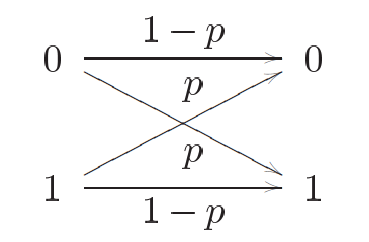
\includegraphics[width=0.3\textwidth]{images/classical_noise.png}
    \caption{A bit flip might occur with probability $p$}
    \label{fig:classical_noise}
\end{figure}
To figure out this probability $p$, we need to understand two things \begin{enumerate*}[label=(\alph*)]
\item How the magnetic fields are distributed in the enviroment. Assuming the owner isn't crazy and placing a magnet near the disk, we can sample the magnetic field near the disk similar to the one the disk is in.
\item How this environment's magnetic field interacts with the disk. This can be done by the well established \textit{Maxwell's equations}.
\end{enumerate*}

Suppose $p_0$, $p_1$ be the probabilities that the bit is in state 0 and 1 initially. Let $q_0, q_1$ be the corresponding probabilities after the noise has occured and $X, Y$ be the initial and final states respectively then
\begin{equation}
    P(Y=y) = \sum_x P(Y=y | X=x)P(X=x)
\end{equation}
where the conditional probability $P(Y=y | X=x)$ is known as the \textit{transition probability}. Thus
\begin{equation}
    \begin{bmatrix}
        q_0 \\ q_1
    \end{bmatrix}
    = \begin{bmatrix}
        1-p & p \\ p & 1-p
    \end{bmatrix}
    \begin{bmatrix}
        p_0 \\ p_1
    \end{bmatrix}
\end{equation}
Suppose we make a quantum circuit made of two faulty \textsc{not} gates. It takes an input state $X$ converts it into an intermediate bit $Y$ which is finally converted to $Z$. If we make a physically reasonable assumption that the noise produced at first \textsc{not} gate independent of the noise produced at the second \textsc{not} gate, it results in a stochastic process $X\longrightarrow Y\longrightarrow Z$ of a special type known as \textit{Markov process}. Often in multi-stage processes, it's a good assumption to use Markov processes. 

For a single stage process, output probabilities $\vv{q}$ are related to the input probabilities $\vv{p}$ according to
\begin{equation}
    \vv{q} = E\vv{p}
\end{equation}
$E$ is a matrix of transition probabilities known as the \textit{Evolution matrix}. Thus the final state of system is linearly related to it's initial state. This linearity is echoed in quantum noise's description, where probability distributions are replaced by density operators. In addition to this, $E$ follows two more rules
\begin{enumerate*}[label=(\alph*)]
    \item All of it's entries must be positive, so that $E\vv{p}$ is also positive and a valid probability distribution. This is known as \textit{positivity}.
    \item Sum of the entries in each column should be 1. This is known as \textit{completeness}.
\end{enumerate*}

\section{Quantum operations}
\subsection{Overview}
Quantum operations formalism is a general tool for describing evolution of quantum systems in a wide variety of circumstances, include stochastic changes, similar to how Markov processes describing classical stochastic changes. Similar to how classical bits are represented using probability distributions, here we'll use \textit{density operators}. The transformation looks like
\begin{equation}
    \rho' = \mathcal{E} (\rho)
\end{equation}
Here, $\rho$ is the initial density operator describing the state of the system. Similarly, $\rho'$ is the final state upto a normalization factor. A few known transforms $\mathcal{E}$ are unitary transformations and measurements $\mathcal{E}(\rho) = U\rho U^\dag$ and $\mathcal{E}_m(\rho) = M_m\rho M_m^\dag$.

In our further study, we're going to look at quantum operations \textit{three} seperate ways. The first way is based on the idea of studying dynamics as the result of interaction between a system and environment. This method is \textit{concrete} and easy to relate to real world. But it is mathematically inconvenient. Second way is euivalent to the first one but is mathematically convenient using a powerful mathematical representation for quantum operations known as the \textit{operator-sum representation}. Third way is equivalent to the first two, it's via a set of \textit{physically motivated axioms} that we'd expect these maps to satisfy. It's advanage is that it shows that quantum dynamics will be described by quantum operations in a wide range of circumstances. But this is neither concrete nor mathematically convenient. 
\begin{figure}[H]
    \centering
    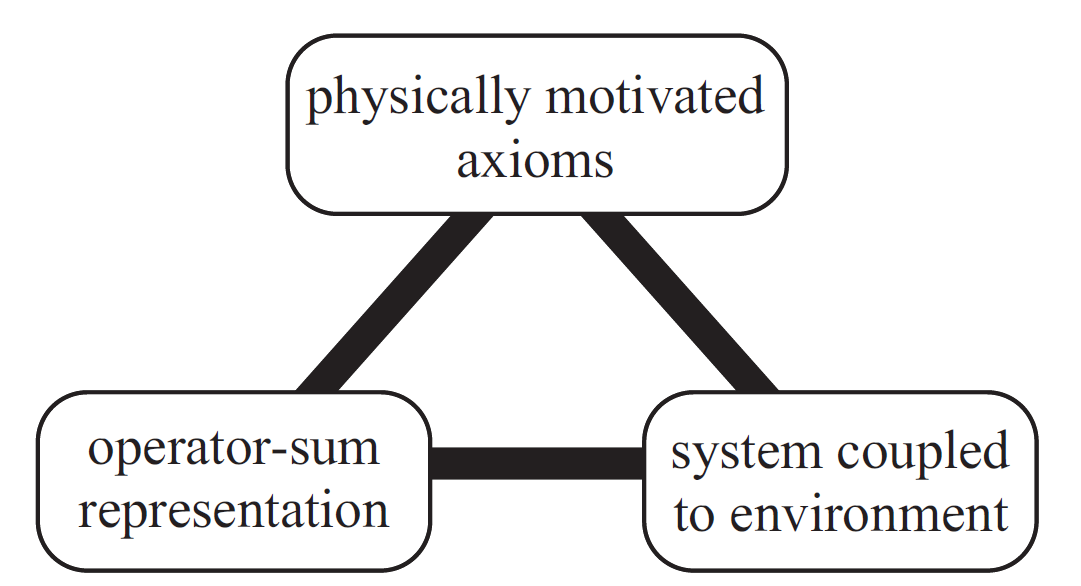
\includegraphics[width=0.6\textwidth]{images/quantum_operations.png}
    \caption{Three ways we're going to look at quantum operations, each provide their own advantages}
    \label{fig:quantum_operations}
\end{figure}

\subsection{Environment and quantum operations}
By the postulate of quantum mechanics, dynamics of a \textit{closed} system is described by just a unitary transform which can be thought of as a box. For dynamics of an \textit{open} system, the system can be thought of as a composite closed system of the system we're considering, \textit{principal system} and the \textit{environment}. 

Suppose the system is in state $\rho$, then the final state would be $\mathcal{E}(\rho)$ which need not be a unitary transform. We \textit{assume} that system and environtment are in a product state $\rho \otimes \rho_{env}$. Evolution of this closed system is described by a unitary transform $U$ and we use partial trace to find final state of the system $\mathcal{E}(\rho)$
\begin{equation}
    \mathcal{E}(\rho) = \text{tr}_{\text{env}} \left[ U\rho \otimes \rho_{\text{env}} U^\dag \right]
\end{equation}
This is the first \textit{definition} of quantum operations. If $U$ doesn't depend on the environment, then final state is simply $\Tilde{U}\rho \Tilde{U}^\dag$ where $\Tilde{U}$ is just part of transform on our principal state.

We assumed that environment and principal system are in a product state, but this might not be the case always. In cases of practical interest, this assumption is reasonable. The experimentalist while preparing an open state clears all the \textit{correlations} between the state and environment.

You might thin the envionment would have near-infinite dimensional Hilbert space, but it turns out that for principal system with $d$-dimensional Hilbert space, it's enough to model the environment with no more that $d^2$ dimensions.

\subsection{Operator sum representation}
How an open system evolves can be understood with an operator acting on the Hilbert space of principal system. This representation of quantum operations is known as \textit{Operator sum representation}.

Let this environment be in a pure state $\rho_{\text{env}} = \op{e_0}$, which even if it's not, can be made pure. Let $\ket{e_k}$ be an orthonormal basis for environment. The operation can be represented as
\begin{align}
    \mathcal{E}(\rho) &= \sum_k \bra{e_k} U\left[ \rho \otimes \op{e_0}) \right] U^\dag \ket{e_k} \\
    &= \sum_k E_k \rho E_k^\dag
\end{align}

where $E_k = \bra{e_k} U \ket{e_0}$ is an operator acting on principal state known as an \textit{operation element.} These have a nice property known as \textit{completeness relation} coming from the fact that $\tr{\mathcal{E}(\phi)} = 1$ since that's just another valid state
\begin{align}
    1 &= \tr{\mathcal{E}(\rho )} \\
    &= \text{tr}\left( \sum_k E_k \rho E_k^\dag \right) \\
    &= \text{tr} \left( \sum_k E_k E_k^\dag \rho \right)
\end{align}
As it's true for all $\rho$,
\begin{equation}
    \sum_k E_k E_k^\dag = I
\end{equation}
This is satisfied by operations which are \textit{trace-preserving}. We'll see later non trace preserving operations are also equivalent to this.

This representation gives us \textit{intrinsic} means to characterize dynamics of the principal system. We don't need to know how the environment works, just $E_k$ are sufficient.
Next up we'll see it's physical interpretation, making a physical model from this representation and also how to define this representation when our assumptions faii.

\subsubsection{Physical inerpretation of operator-sum representation}
Suppose a unitary transform $U$ is applied followed by a measurement of the environment, in basis $\ket{e_k}$. The measurement only affects the environment, thus state of the system if the output is $k$ is
\begin{align}
    \rho_k &\propto \text{tr}_E\left( \op{e_k}U(\rho \otimes \op{e_0}) U^\dag \op{e_k} \right) \\
    &= \bra{e_k} U\left( \rho \otimes \op{e_0}) \right) U^\dag \ket{e_k} \\
    &= E_k \rho E_k^\dag
\end{align}
which upon normalizing gives,
\begin{align}
    \rho_k = \frac{E_k\rho E_k^\dag}{\tr{E_k\rho E_k^\dag}}
\end{align}
with probability
\begin{equation}
    \tr{E_k\rho E_k^\dag}
\end{equation}
thus the final output is
\begin{align}
    \mathcal{E}(\rho) = \sum_k E_k\rho E_k^\dag
\end{align}

Thus we can see that a quantum operation changes the input randomly into a state $\frac{E_k\rho E_k^\dag}{\tr{E_k\rho E_k^\dag}}$ with probability $\tr{E_k\rho E_k^\dag}$ which is very similar to a noisy channel.

\subsubsection{Measurement and operator-sum representation}
We can have non trace preserving operations if we allow \textit{measurement} of the prinicpal state-environment system after the operator $U$ is applied. Suppose the principal system is represented by $Q$ and the environment by $E$, both are initially independent, environment is in the state $\sigma$. Then
\begin{equation}
    \rho^{QE} = \rho \otimes \sigma
\end{equation}
Now a unitary transform $U$ is applied, then a projective measurement is made using $P_m$. We assume no measurement is made is same as the outcome is $m=0$ and $P_0\equiv I$. The final state of $QE$ is
\begin{equation}
    \frac{P_m U(\rho \otimes \sigma) U^\dag P_m}{\tr{P_m U(\rho \otimes \sigma) U^\dag P_m}}
\end{equation}
State of only the principal system $Q$ is
\begin{equation}
    \frac{\text{tr}_E(P_m U(\rho \otimes \sigma) U^\dag P_m)}{\tr{P_m U(\rho \otimes \sigma) U^\dag P_m}}
\end{equation}
We can define a map $\mathcal{E}_m(\rho)$ as
\begin{equation}
    \mathcal{E}_m(\rho) = \text{tr}_E(P_m U(\rho \otimes \sigma) U^\dag P_m)
\end{equation}
therefore the final state of $Q$ is $\frac{\mathcal{E}_m(\rho)}{\tr{\mathcal{E}_m(\rho)}}$ and $\tr{\mathcal{E}_m(\rho)}$ is the probability of measurement outcome $m$. Suppose $\ket{e_k}$ is an orthonormal basis of $E$ and $\sigma=\sum_j q_j\ket{j}$ is an ensemble of initial state of environment then we observe that
\begin{align}
    \mathcal{E}_m(\rho) &= \sum_{jk} q_j\text{tr}_E(\op{e_k}P_m U(\rho \otimes \sigma) U^\dag P_m\op{e_k}) \\
    &= \sum_{jk} E_{jk} \rho E_{jk}^\dag
\end{align}
where
\begin{equation}
        E_jk \equiv \sqrt{q_j}\bra{e_j}U\ket{j}
\end{equation}
using which we can calculate the operators for the operator sum representation if $\sigma$ of $E$ is known. Even though we don't make projective measurements, respective measurement probabilities are $\tr{\mathcal{E}_m(\rho)}$

\subsubsection{System-environment models for any operator-sum representation}
Now a natural question is for a given set of operators $\{ E_k \}$ is it possible to find a reasonable \textit{model environment system and dynamics} which give rise to the quantum operation described by these operators. It turns out that for a set of trace preserving or non trace preserving quantum operation $\mathcal{E}$, there exists a model environment $E$ staring with a pure state $\ket{e_0}$, and model dynamics specified by unitary operator $U$ and projector $P$ onto $E$ such that
\begin{equation}
    \mathcal{E}(\rho) = \text{tr}_E(PU(\rho \otimes \op{e_0})U^\dag P)
\end{equation}

\subsection{Axiomatic approach to quantum operations}
We'll try to write down physically motivated axioms which quantum operations obey. We'll start over from scratch using these axioms. We'll then prove that a map $\mathcal{E}$ satisfies these axioms \textit{if and only if} it has an operator sum representation.

We \textit{define} a quantum operation $\mathcal{E}$ as a map from the set of density operators of the input space $Q_1$ to the set of density operators for the output space $Q_2$, which satisfy the following (for convenience we'd take $Q_1=Q_2=Q$):
\begin{enumerate}
    \item $\tr{\mathcal{E}(\rho)}$ denotes the probability that the map described by $\mathcal{E}$ occurs. Thus $0 \leq \tr{\mathcal{E}(\rho)} \leq 1$.
    \item $\mathcal{E}$ is a \textit{convex-linear map} on the set of density matrices i.e
    \begin{equation}
        \mathcal{E}\left( \sum_i p_i\rho_i \right) = \sum_i p_i\mathcal{E}(\rho_i).
    \end{equation}
    \item $\mathcal{E}$ is a \textit{completely-positive map} i.e $\mathcal{E}(A)$ is positive for any positive $A$. Also, if we introduce an extra system $\mathcal{R}$, then $\mathcal{I}\otimes \mathcal{E}(A) $ is positive for any positive $A$ in $\mathcal{R}Q_1$, where $\mathcal{I}$ is the identity map on $\mathcal{R}$.
\end{enumerate}

The following theorem binds the axiomatic approach and the operator-sum representation
\begin{theorem}
    The map $\mathcal{E}$ satisfies the above axioms if and only if
    \begin{equation}
        \mathcal{E}(\rho) = \sum_k  E_k\rho E_k^\dag
    \end{equation}
    for some set of operators $\{ E_k \}$ mapping the input Hilbert space to the output Hilbert space and satisfying $\sum_k E_k E_k^\dag \leq I$
\end{theorem}

\subsubsection{Freedom in the operator-sum representation}
A quanum operation can be described by two different set of operators. For example take $\mathcal{E}(\rho)=\sum_k E_k\rho E_k^\dag$ and $\mathcal{F}(\rho) = \sum_k F_k\rho F_k^\dag$ and
\begin{align}
    E_1 &= \frac{I}{\sqrt{2}} = \frac{1}{\sqrt{2}}\begin{bmatrix}
        1 & 0 \\ 0 & 1
    \end{bmatrix}
    &E_2 = \frac{Z}{\sqrt{2}} = \frac{1}{\sqrt{2}}\begin{bmatrix}
        1 & 0 \\ 0 & -1
    \end{bmatrix}
    \\
    F_1 &= \op{0} = \begin{bmatrix}
        1 & 0 \\ 0 & 0
    \end{bmatrix}
    &F_2 = \op{1} = \begin{bmatrix}
        0 & 0 \\ 0 & 1
    \end{bmatrix}
\end{align}

Understanding which sets of operations gives rise to same quantum operations is important for two reasons. \begin{enumerate*}[label=(\alph*)]
    \item Understanding the freedom in representation gives us more insight into how different physical processes give rise to same dynamics
    \item Understanding freedom in operator-sum representation is cruicial to a good understanding of quantum error-correction.
\end{enumerate*}
This is described usin the following theorem
\begin{theorem}[\textbf{Unitary freedom in the operator-sum representation}]
    Suppose $\{ E_1,\cdots, E_m \}$ and $\{ F_1, \cdots, F_n \}$ are operation elements giving rise to quantum operations $\mathcal{E}$ and $\mathcal{F}$ respectively. We may ensure $m=n$ by appending 0 operators to the end of shorter operation elements' list. Then $\mathcal{E}=\mathcal{F}$ if and only if there exist complex numbers $u_{ij}$ such that $E_i = \sum_j u_ij F_j$ and $u_{ij}$ is a unitary matrix.
\end{theorem}

This is similar to the result when two states are denoted by the same density operator. Using this theorem we can also answer the question, what is the maximum number of dimensions of an environment needed to mock up a quantum operation as described by this theorem.

\begin{theorem}
    All quantum operations $\mathcal{E}$ on a principal system of Hilbert space dimension $d$ can be generated by an operator sum representation containing atmost $d^2$ elements, i.e
    \begin{equation}
        \mathcal{E}(\rho) = \sum_{k=1}^M E_k\rho E_k^\dag
    \end{equation}
    where $1\leq M\leq d^2$.
\end{theorem}

\section{Examples of quantum noise and quantum operations}
\subsection{Trace and partial trace}
Quantum operations formalism can be used to describe a measurement, it's outcome and the state of the system after the measurement. The simplest such operation is related to the map $\rho \longrightarrow \tr{\rho}$. Let $H_Q$ be the input Hilbert space with orthogonal basis $\ket{1}, \cdots, \ket{d}$ and $H_Q'$ is a one dimensional Hilbert space, spanned by $\qo$, define $\mathcal{E}(\rho)$ as
\begin{equation}
    \mathcal{E}(\rho) \equiv \sum_{i=1}^{d} \qo \bra{i} \rho \ket{i} \bra{0}
\end{equation}
Do note that $\mathcal{E}(\rho) = \tr{\rho}\op{0}$, thus this quantum operation is identical to the trace operation, ignoring the factor of $\op{0}.$

Another interesting thing comes when we have a joint system $QR$ and we want to trace out $R$. Let $\ket{j}$ be the basis of $R$, let's define a linear operator $E_i: H_{QR} \longrightarrow H_Q$ as
\begin{equation}
    E_i\left( \sum_j \lambda_j \ket{q_j} \ket{j} \right) = \lambda_i \ket{q_i}
\end{equation}
when $\ket{q_j}$ are arbitrary vectors in $Q$ and $\lambda_j$ are just constants. Then we define a quantum operation as
\begin{equation}
    \mathcal{E}(\rho) \equiv \sum_k E_k\rho E_k^\dag
\end{equation}
We also notice that
\begin{equation}
    \mathcal{E}(\rho \otimes \ket{j}\bra{j'}) = \rho \delta_{j, j'} = \rho \tr{\ket{j}\bra{j'}} = \text{tr}_R(\rho \otimes \ket{j}\bra{j'}).
\end{equation}
where $\ket{j}, \ket{j'}$ are members of orthonormal basis of $R$. Thus, by linearity of $\mathcal{E}$ and $\text{tr}_R$ we have $\mathcal{E} = \text{tr}_R$
\subsection{Geometric picture of single qubit quantum operations}
We've seen before that a single qubit's density operator can be represented by
\begin{equation}
    \rho = \frac{I+\Vec{r} \cdot \Vec{\sigma}}{2}
\end{equation}
where $\Vec{r}$ is a three dimensional real unit vector and $\Vec{\sigma}$ is a vector of pauli matrices. Thus
\begin{equation}
    \rho = \frac{1}{2}\begin{bmatrix}
        1+r_z & r_x-ir_y \\ r_x+ir_y & 1-r_z
    \end{bmatrix}
\end{equation}
Using this representation, it can be shown that an arbitrary trace-preserving quantum operation is equivalent to the map
\begin{equation}
    \Vec{r} \longrightarrow \Vec{r}' = M\Vec{r} + \Vec{c}
\end{equation}
where $M$ is a $3\times 3$ real matrix, and $\Vec{c}$ is a constant vector. This is an \textit{affine map}, mappping Bloch sphere into itself. To see this, suppose the operators $E_i$ generating $\mathcal{E}$ are written in the form
\begin{equation}
    E_i = \alpha_i I + \sum_{k=1}^3 a_ik\sigma_k
\end{equation}
Then it can be checked that
\begin{align}
    M_{jk} = \sum_l \left[ a_{lj}a_{lk}^* + a_{lj}^*a_{lk} + \left( |\alpha_l|^2 - \sum_p a_{lp}a_{lp}^* \right) \delta_{jk} + i\sum_p \epsilon_{jkp}(\alpha_la_{lp}^* - \alpha_l^*a_{lp}) \right] 
\end{align}
\begin{align}
    c_k = 2i \sum_l \sum_{jp}\epsilon_{jpk}a_{lj}a_{lp}^*
\end{align}
The affine map can be better understood by te polar decomposition of $M$ into $M=U|M|$, where $U$ is unitary. Since $M$ is real, $|M|$ is real and hermitian, i.e a symmetric matrix. Thus, as $M$ is real, we may assume $U$ is real, and an orthogonal matrix i.e $U^TU=I$ Thus, we can write
\begin{equation}
    M = OS
\end{equation}
where determinant of $O$ is 1 and it's an orthogonal matrix describing rotation. $S$ is a real symmetric matrix. Thus the above equation can be understood as the deformation of the bloch sphere about axis as specified by $S$ followed by a rotation defined by $O$, then a displacment due to $\Vec{c}$.
\subsection{Bit flip and phase flip channels}
Suppose we take a single qubit and pass it through a noisy \textit{bit-flip} channel, which flips the state of a qubit from $\qo$ to $\qi$ with probability $1-p$. It has operation elements
\begin{align}
    &E_0 = \sqrt{p}I = \sqrt{p}\begin{bmatrix}
        1 & 0 \\ 0 & 1
    \end{bmatrix}
    &E_1 = \sqrt{1-p}X = \sqrt{1-p}\begin{bmatrix}
        0 & 1 \\ 1 & 0
    \end{bmatrix}
\end{align}
This affects the bloch vector in the following way:
\begin{figure}[H]
    \centering
    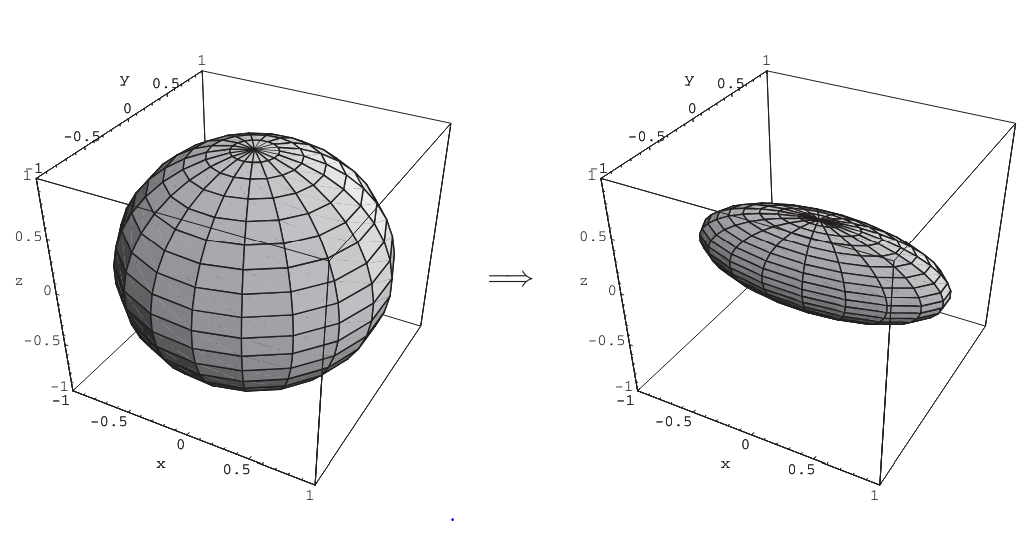
\includegraphics[width=\textwidth]{images/bit_flip_bloch.png}
    \caption{Bit flip channl. The operation doesn't affect the $x$ component, but shrinks the $y$ and $z$ component by a factor of $1-2p$. Here $p=0.3$.}
    \label{fig:bit_flip_bloch}
\end{figure}
It's easy to verify that $\tr{\rho^2}=\frac{1+|\Vec{r}|^2}{2}$. Thus, this operation can never increase the length of Bloch vector i.e can never increase $\tr{\rho^2}$. Thus the purity of $\rho$ is always decreased by this. Thus Bloch sphere provides an intuitive way of understanding quantum operations.   

Similarly if we consider the \textit{phase-flip} channel which has operation elements
\begin{align}
    &E_0 = \sqrt{p}I = \sqrt{p}\begin{bmatrix}
        1 & 0 \\ 0 & 1
    \end{bmatrix}
    &E_1 = \sqrt{1-p}Z = \sqrt{1-p}\begin{bmatrix}
        1 & 0 \\ 0 & -1
    \end{bmatrix}
\end{align}
we see that the following transformation is happening to the Bloch sphere.
\begin{figure}[H]
    \centering
    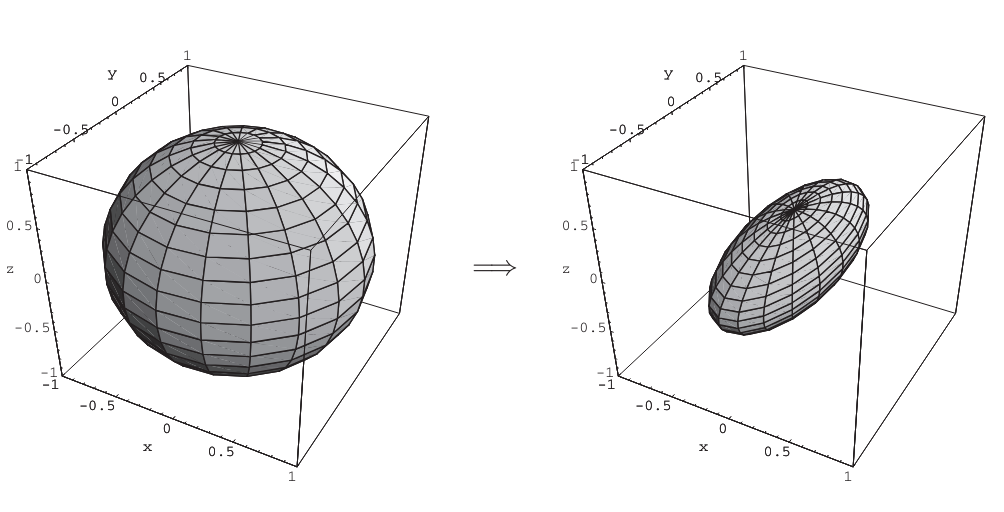
\includegraphics[width=\textwidth]{images/bit_phase_flip_bloch.PNG}
    \caption{Phase flip channel. As we can see, it does nothing to the $z$ component, but shrinks $x$ and $y$ component by a factor of $1-2p$. Here p=0.3.}   
    \label{fig:phase_flip_bloch}
\end{figure}
As a special case when $p=0.5$, using the freedom in the operator-sum representation, this operation can be written as
\begin{equation}
    \rho \longrightarrow \mathcal{E}(\rho) = P_0\rho P_0 + P_1\rho P_1
\end{equation}
which is nothing but the measurement with respect to the basis $\qo, \qi$, the result unknown. The corresponding map on Bloch sphere here is 
\begin{equation}
    (r_x,r_y,r_z) \longrightarrow (0,0,r_z)
\end{equation}
i.e the Bloch vector is projected along $z$ axis loosing $x$ and $y$ components.

The \textit{bit-phase flip} channel has the operation elements
\begin{align}
    &E_0 = \sqrt{p}I = \sqrt{p}\begin{bmatrix}
        1 & 0 \\ 0 & 1
    \end{bmatrix}
    &E_1 = \sqrt{1-p}Y = \sqrt{p}\begin{bmatrix}
        0 & -i \\ i & 0
    \end{bmatrix}
\end{align}
when this operation is done, the $y$ component of the Bloch sphere remain intact. Whereas $x,z$ components are shrinked by a factor of $1-2p$ as shown
\begin{figure}[H]
    \centering
    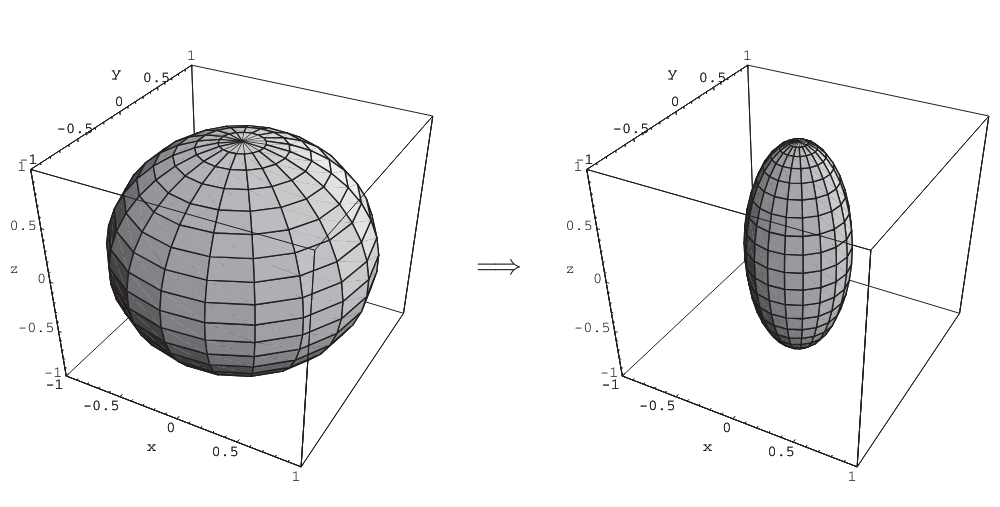
\includegraphics[width=\textwidth]{images/phase_flip_bloch.PNG}
    \caption{Bit-phase flip channel. Here p=0.3, it can e seen that $y$ axis remains intact while $x$ and $z$ axes are shrinked by a factor of $1-2p$.}
    \label{fig:bit_phase_flip_bloch}
\end{figure}
\subsection{Depolarizing channel}
It's an important type of quantum noise channel. We take a single qubit, and with probability $p$ the qubit is \textit{depolarized} i.e replaced by a completely mixed state $\frac{I}{2}$ or left untouched with probability $1-p$. Thus the state of the qubit after noise is
\begin{equation}
    \E{\rho} = \frac{pI}{2} + (1-p)\rho
    \label{eq:depolarizing_channel}
\end{equation}
The effect on Bloch sphere is as shown
\begin{figure}[H]
    \centering
    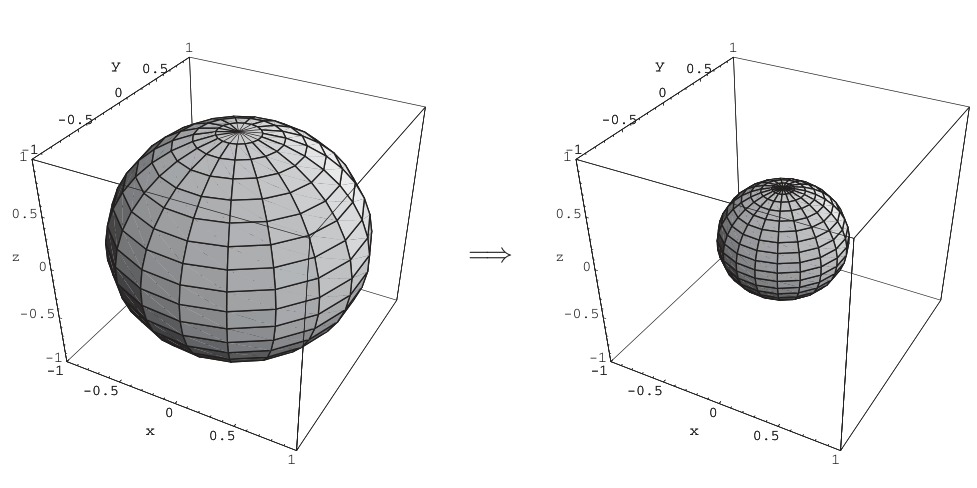
\includegraphics[width=0.9\textwidth]{images/depolarizing_bloch.png} 
    \caption{Effect of depolarizing channel on the Bloch sphere}
    \label{fig:depolarizing_bloch}
\end{figure}
The quantum circuit depicting the depolarizing channel is
\begin{figure}[H]
    \centering
    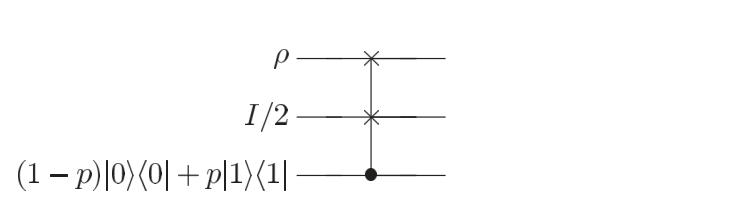
\includegraphics[width=0.7\textwidth]{images/depolarizing_circuit.png}
    \caption{Quantum circuit representing the depolarizing channel}
    \label{fig:depolarizing-circuit}
\end{figure}
The third qubit is qubit is a mixture of state $\qo$ and $\qi$ with probability $p$ and $1-p$ respectively. This is responsible for the second qubit getting swapped into the first qubit. In \ref{eq:depolarizing_channel}, $I/2$ can be represented as
\begin{equation}
    \frac{I}{2} = \frac{\rho + X \rho X + Y \rho Y + Z \rho Z}{4}
\end{equation}
Thus \ref{eq:depolarizing_channel} becomes
\begin{equation}
    \E{\rho} = \left( 1-\frac{3p}{4} \right) \rho + \frac{p}{4}\left( X \rho X + Y \rho Y + Z \rho Z \right)
\end{equation}
Here the operation elements will be $\sqrt{1-3p/4}I$, $\sqrt{p}X/2$, $\sqrt{p}Y/2$, $\sqrt{p}Z/2$. Note that it is convenient to parametrize the depolarizing channel in different ways. The operation elements would differ, such as
\begin{equation}
    \E{\rho} = (1-p)\rho + \frac{p}{3}\left(X \rho X + Y \rho Y + Z \rho Z \right)
\end{equation}
Here, this does nothing with probability $1-p$ and applies $X$, $Y$ or $Z$ gates with probability $p/3$ each.

The depolarizing channel can be generalized for systems with dimensionality greater than 2. Suppose a system has dimension $d$ the quantum operation would become
\begin{equation}
    \E{\rho} = \frac{pI}{d} + (1-p)\rho
\end{equation}
\subsection{Amplitude damping}
The process of \textit{amplitude damping} helps us understand \textit{energy dissipation} in quantum systems. For example, to describe dynamics of an atom emitting a photon, how a spin system at high temperature reaches equilibrium with it's environment etc. What's common in these examples is described by a quantum operation known as \textit{amplitude damping}, which can be derived as follows. Suppose we have an optical mode at state $a\qo+b\qi$ which is superposition of zero or one photon. The scattering of a photon can be now described as keep a partially silvered mirror (a beamsplitter) in the path of the photon. It couples with another single optical node (it's environment) according to unitary transform $B = \exp{\left[ \theta(a^\dag b - ab^\dag \right]}$. Where $a$, $a^\dag$ and $b$, $b^\dag$ are annihilation and creation operators for photons in two modes. The output after beamsplitter assuming there's no photon in the environment is $B\qo(a\qo+b\qi) = a\ket{00} + b(\cos{\theta}\ket{01} + \sin{\theta}\ket{10}$. Tracing out the environment gives us the quantum operation
\begin{equation}
    \mathcal{E}_{AD}(\rho) = E_0\rho E_0^\dag + E_1\rho E_1^\dag
\end{equation}
where $E_k=\bra{e_k}0\ket{e_0}$ are
\begin{align}
    E_0 &= \begin{bmatrix}
        1 & 0 \\ 0 & \sqrt{1-\gamma}
    \end{bmatrix} \\
    E_1 &= \begin{bmatrix}
        0 & \sqrt{\gamma} \\ 0 & 0
    \end{bmatrix},
\end{align}
the operations elements for amplitude damping. $\gamma = \sin^2(\theta)$ can be thought of as the probability of loosing a photon. $E_1$ operation changes the state $\qi$ to $\qo$, this corresponds to the loss of quantum of energy to the environment. $E_0$ leaves $\qo$ unchanged but reduces the amplitude of $\qi$, this happens because there's no loss of quantum of energy, thus the environment perceives it to be more likely that the system is in $\qo$ state.
\begin{figure}[H]
    \centering
    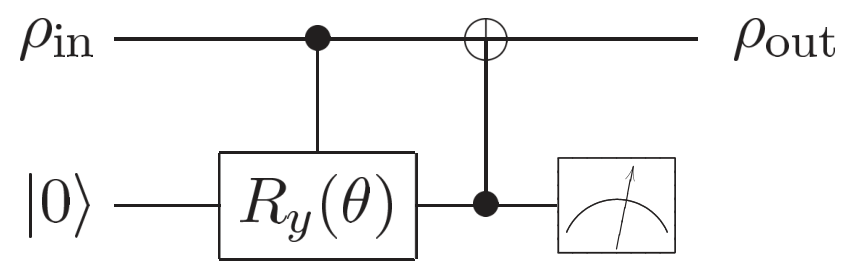
\includegraphics[width=0.6\textwidth]{images/amplitude_damp_circuit.png}
    \caption{This models an amplitude damping circuit with $\gamma = \sin^2(\theta/2)$}
    \label{fig:amplitude_damp_circuit}
\end{figure}
A general characteristic of a quantum operation is the set of states that are left invariant under the operation, as we've seen before. Here, $\qo$ is left invariant, but that is a cause of us assuming that the environment is starting at $\qo$ state, as if it were at \textit{zero temperature}.

The quantum operation defining amplitude damping at a finite temperature is known as \textit{generalized amplitude damping}, $\mathcal{E}_{\text{GAD}}$ and is defined for single qubits using operation elements
\begin{align}
    E_0 &= \sqrt{p}\begin{bmatrix}
        1 & 0 \\ 0 & \sqrt{1-\gamma}
    \end{bmatrix}
    &E_1 = \sqrt{p}\begin{bmatrix}
        0 & \sqrt{\gamma} \\ 0 & 0
    \end{bmatrix}
    \\
    E_2 &= \sqrt{1-p}\begin{bmatrix}
        \sqrt{1-\gamma} & 0 \\ 0 & 1
    \end{bmatrix}
    &E_3 = \sqrt{1-p}\begin{bmatrix}
        0 & 0 \\ \sqrt{\gamma} & 0
    \end{bmatrix}
\end{align}
and the stationary state $\rho_\infty$ satisfies $\E{\rho_\infty} = \rho_\infty$. This  GAD describes `$T_1$' relaxation processes due to coupling of spin to their surrounding lattice, a large system which is in thermal equilibrium at a temperature much higher than the spin temperature. This thing is useful in NMR quantum computation.

The effect of amplitude damping on Bloch sphere is 
\begin{equation}
    (r_x, r_y, r_z) \longrightarrow \left(r_x\sqrt{1-\gamma}, r_y\sqrt{1-\gamma}, \gamma+r_z(1-\gamma)\right)
\end{equation}
where $\gamma$ is replaced with a time varying function like $1-e^{-t/T_1}$ ($t$ is time and $T_1$ characterizes speed of the process). Using this we can visualize the effects as \textit{flow} on the Bloch sphere, where every point moves towards a fixed point, something like north pole where $\qo$ is located.

Similarly, generalized amplitude damping performs the transformation
\begin{equation}
    (r_x, r_y, r_z) \longrightarrow \left( r_x\sqrt{1-\gamma}, r_y\sqrt{1-\gamma}, \gamma(2p-1) + r_z(1-\gamma) \right)
\end{equation}
Generalized ammplitude damping is different than amplitude damping only in the location of fixed point of flow; the final state is along $\hat{z}$ axis, at the point $(2p-1)$, which is a mixed state.
\begin{figure}[H]
    \centering
    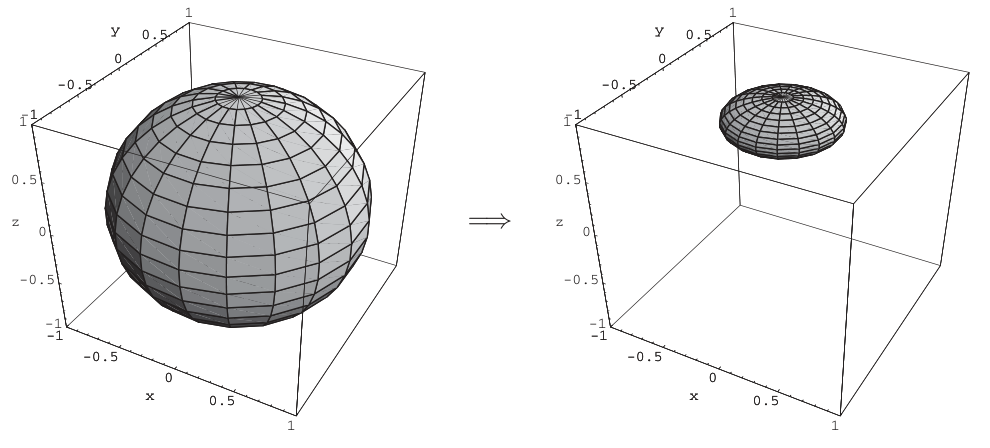
\includegraphics[width=\textwidth]{images/gad_bloch.png}
    \caption{The effect of amplitude damping channel on Bloch sphere, for $p=0.8$. Note how the entire sphere shrinks towards the north pole, the $\qo$ state.}
    \label{fig:gad_bloch}
\end{figure}

\subsection{Phase damping}
A noise process which is uniquely quantum mechanical, describes \textit{loss of quantum information} without \textit{loss of energy}, is \textit{\textbf{phase damping}}. For example it describes what happens when a photon scatters randomly as it travels through a waveguide, or how electronic states in an atom are perturbed upon interacting with distant electrical charges. The energy eigenstates don't change as a function of time but accumulate a phase proportional to the eigenvalues. When a system evolves for an amount of time not known, information about this quantum phase - the \textit{relative} phases between the eigenstates is lost.